\section{Outils mis en place}

\begin{itemize}
	\item Site web en ligne (CMS Wordpress): \url{http://www.ecole.ensicaen.fr/~lvimont/} 

		\begin{figure}[h!]
			\centering
			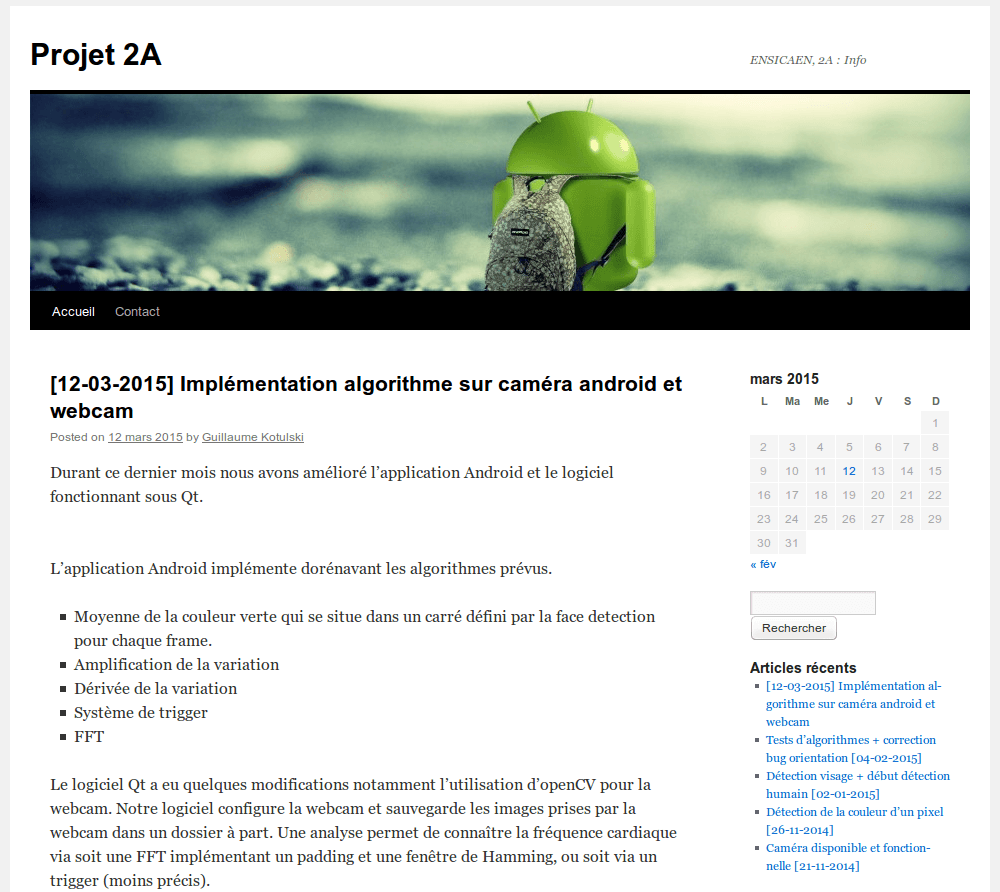
\includegraphics[width=0.9\textwidth]{data/website.png}
			\caption{Capture d'écran du site web.}
		\end{figure}

	\item Gestionnaire de versions (Git) 
		\begin{itemize}[label=\textbullet]
			\item Application Android: \url{https://github.com/F4r3n/Vamp} 
			\item Logiciel de traitement d'images: \url{https://github.com/F4r3n/ImageProject.git} 
		\end{itemize}
	\item Gestionnaire de projet (Trello)
\end{itemize}

\section{Technologies utilisées}

\begin{itemize}[label=\textbullet]
	\item Java 
	\item C++
	\item QT
	\item Android
	\item OpenCV 
\end{itemize}

\section{Algorithme mis en place}

L'oeil humain est limité, en effet il est incapable de voir les subtils changements temporels. Alors
que justement en effectuant des traitements sur une vidéo. On est capable de révéler ces changements
comme par exemple, la circulation du sang. On peut même grâce à ça réussir à connaitre le pouls d'une
personne. 

Notre première idée fut simplement de réaliser une moyenne pour chaque couleur pour un pixel, puis 
une moyenne de tout les moyennes calculer par pixels. On pensait alors par la suite grâce à cette 
collection de moyenne arriver a détecter une variation. En effectuant par exemple, une dérivée puis
une amplification de la courbe obtenue.  

Dans un second temps, en restant basé sur le même principe, nous avons tenté de découper notre image
par zone de petits carrés de pixels. Par exemple une zone serait d'une taille de 5*5. On réalise 
ainsi une moyenne de chaque zone, puis par la suite une moyenne de ces moyennes. Enfin on réapplique
les mêmes fonctions qu'au-dessus.

\section{Solutions mis en place}

Durant le projet nous avons développés plusieurs outils pour répondre au besoin. Une application Android qui permettrait d'utiliser le moyen d'authentification désiré et ainsi déverouiller le smarthpone d'une
personne. Un logiciel C++ utilisant la librairie QT a également été mis en place, afin de pouvoir tester plus facilement les algorithmes que nous voulions développer. Dans la suite du projet, il a également
permis d'utiliser la webcam. 

\subsection{Développement Android}

	Notre application Android est capable d'utiliser la caméra frontale de n'importe quel smartphone. L'api d'android propose une classe appelée FaceDetectionListener qui va permettre de capter, les visages présent 
	devant une caméra, grâce à ce système il est possible de dessiner un Rect (c'est à dire un rectangle) autour du visage de la personne. C'est notre classe DisplayedFace qui se charge de ce travail. Une fois la 
	reconnaissance mis en place, nous avons utiliser la fonction \href{http://developer.android.com/reference/android/hardware/Camera.PreviewCallback.html#onPreviewFrame\%28byte\%5B\%5D,\%20android.hardware.Camera\%29}{onPreviewFrame}. Cette dernière permet d'enregistrer en temps réel, les données. On lance un compteur quand la première reconnaissance d'un visage a lieu, ce dernier va durer 5 secondes.\\
\\
	Les données ainsi récoltées sont au format de l'espace de couleur \href{http://fr.wikipedia.org/wiki/YUV}{YUV}. Nous devons donc convertir ces données au format RGB qui se révèle plus évocateur au niveau des variations. 
	A la fin du compteur, on réalise une dérivée, puis une amplifaction des valeurs obtenues. On observe alors les variations qu'on obtient et on conclu alors sur la présence ou non d'un humain.

\subsection{Développement C++}

	Nous avons créé un logiciel C++ nous permettant de tester nos algorithmes avant de les implémenter sous Android.
	Ce logiciel a de nombreuses fonctionnalitées, notamment le découpage d'une vidéo en images pour permettre une analyse plus poussée.
	Nous utilisons avconv qui permet de découper une vidéo de n'importe quelle taille en une multitude d'images (15 images * taille de la vidéo)
	Après avoir découpé la vidéo en images nous faisons une analyse sur ces images.
	Cette analyse se découpe en plusieurs étapes.
	Dans un premier temps nous dessinons un rectangle autour d'un visage (si la fonction du rectangle automatique n'est pas enclenchée)
	Puis nous choisissons le type d'analyse a effectué, il y en a deux types:
		-L'une fait la moyenne de tous les pixels qui se situe dans le carré
		-La seconde découpe le rectangle en plusieurs zones de 5*5 puis amplifie les variations et fait une moyenne des valeurs
	Après avoir lancé l'analyse, nous affichons les courbes ainsi obtenues par notre application.\\

	Nous pouvons voir la FFT, l'amplification, la dérivée ou une combinaison de plusieurs méthodes.
	L'amplification utilise la dérivée de Taylor du premier degré.
	La FFT utilise un filtre passe-bas combiné avec une fenetre de Hamming et un padding.
	La FFT permet de connaitre le rythme cardiaque d'une personne de manière précise si l'image est assez stable.
	Nous avons créé un Trigger qui permet aussi de connaître la fréquence cardiaque d'une personne mais de manière moins précise, le trigger nous donne une fourchette de valeurs.\\

	Si l'espace de couleur que nous avons choisi ne donne pas des résultats corrects nous pouvons en choisir un autre.
	Nous avons différents espaces de couleur disponible dont RGB, HSL, HUV et nous pouvons lancer une analyse avec un espace de couleur différent de RGB.\\

	Les analyses avec des vidéos classiques n'étant pas suffisantes pour nos tests, nous avons dû faire une analyse avec des vidéos de la webcam.
	La webcam est configurée et lancée via la librairie OpenCV et nous enregistrons les images de la webcam avec une fréquence de 15 frames pas seconde.\\

\section{Problèmes rencontrés}

\subsection{Limitation des sessions à l'ENSICAEN}

Lors du projet, nous avons rencontrés de nombreux problèmes. L'un des plus embêtant est la limite des sessions à l'Ensicaen. En effet, nos sessions dispose du taille limité, nous pouvons uniquement travailler sous Windows (car
c'est seulement sous cet environnement que sont installés les outils android) hors nous disposons d'uniquement 150 Mo, or rien qu'avec firefox, si nous ne nettoyons par régulièrement l'historique, la session se retrouve 
complète. Nous avons malheureument expérimenté le soucis et perdu ainsi, une après midi de travail. 

\subsection{Problèmes rencontrés lors du développement Android}

Nous avons eu un problème de rotation, les coordonnées que l'on converser se révélait mauvaise. On avait en effet un problème de rotation, afin d'éviter cela on force le mode portrait.

La première version de notre application était capable d'enregistrer 15 frames par seconde, or au final on obtenait seulement une trentaine de valeurs, cela était du à la conversion du format YUV au format RGB que l'on 
effectuer à chaque fois que nous rentrons dans la fonction onPreviewFrame, comme la conversion est couteuse O(n\up{2}), on perdait des valeurs. Pour optimiser, le nombre de valeurs nous effectuons maintenant la conversion
une fois le timer fini. On réalise alors dans la boucle une simple sauvegarde des données bruts. 
Toutefois cette méthode, nous a causé pas mal de soucis, notamment des out of memory, c'est à dire, que nous réalisions une allocation trop grande par rapport à la mémoire disponible \ldots{}

% L'incompétence des chercheurs

